\label{cap:semantic_web}
\chapter{Web Semântica}

\begin{quotation}[]{Tim Berners-Lee}
I found myself answering the same questions asked frequently of me by different people. It would be so much easier if everyone could just read my database
\end{quotation}

A introdução e expansão da \textit{World Wide Web} possibilitou acessar e publicar uma grande variedade de conteúdo, seja para o consumo de entretenimento, exposição de opiniões, compras online etc. O crescimento da rede tornou-se tão grande que é latente a dificuldade dos usuários encontrar informações. Para eles, foram criados e desenvolvidos os indexadores de páginas, como o Google\footnote{https://www.google.com}, Yahoo\footnote{https://www.yahoo.com}, Bing\footnote{https://www.bing.com}. Tais sistemas facilitam encontrar informações em serviços populares na Internet. Entretanto, e se quiséssemos encontrar algum médico de confiança para marcar uma consulta, levando em consideração uma agenda de compromissos? Ou então se estamos realizando um trabalho escolar e queremos encontrar os reis do século XV? Essas pesquisas certamente são mais complicadas, e resultados de buscas tradicionais levam a informações fragmentadas, com uma série de outras buscas separadas para alinhar todo o conhecimento e semântica envolvidos nessas tarefas. É nesse ponto que entra o conceito da Web Semântica, como uma extensão da já existente.

O conteúdo da Web tradicional é fundamentalmente desenvolvido para humanos lerem, não para máquinas manipularem de forma produtiva e significante \citep{bernerslee2001semantic}. Originalmente desenvolvida para compartilhar e apresentar conteúdo de forma que fosse possível interagir e navegar entre hipertextos e hipermídia, a \ac{WWW} torna fácil a apresentação de layouts. É possível estruturar um documento com um cabeçalho, um link para outra página, entretanto, dificilmente as máquinas poderão processar semanticamente que informações estão disponíveis e que podem ser organizadas naquela página ou site. Como exemplo, uma página de João com link para seu currículo informando que possui especialização em cardiologia. Todas essas informações podem até serem compreendidas por humanos ao associar a semântica das entidades presentes numa página e analisando links relacionados, mas para a máquina não há uma estrutura comum e eficiente que leve a essas mesmas conclusões.

O objetivo da Web Semântica é de estender a WWW, aproveitando a enorme variedade de dados já existente, mas agregando uma nova camada de metadados que possibilitem o processamento pela máquina e agentes de forma a compreender a semântica das informações apresentadas. Assim, a Web Semântica trata-se de prover formatos para integração de dados de diferentes fontes \citep{SemanticWebW3C}, onde a Web tradicional mantém-se como o meio de publicação e interconexão de documentos, e na contraparte semântica, armazena-se dados que se relacionam com objetos e coisas do mundo real. Um agente pode se deparar com uma página de clínica na Web e não apenas compreenderá que possui palavras como “tratamento, terapia, remédios, médicos”, como tipicamente é encontrado na Web tradicional, mas também saber que o "Dr João" trabalha nessa clínica nas segundas e quartas com horários no formato \textit{dd/mm/YYYY}.

\section{Arquitetura e formato de dados}

O funcionamento da Web Semântica depende da capacidade de máquinas acessar coleções estruturadas de informações, dados e regras de inferência para executar raciocínio automatizado \citep{bernerslee2001semantic}. O desafio é de como representar conhecimento. Inicialmente o desenvolvimento desses sistemas utilizaram uma abordagem centralizadora, requerendo que as partes envolvidas compartilhem exatamente as mesmas definições de conceitos comuns ou hierárquicos. Entretanto, com a quantidade de conteúdo existente hoje em diferentes línguas, controle centralizado é desafiador. Contrastando essa visão inicial, na Web Semântica cria-se linguagens para regras as quais são tão expressivas quanto o necessário para que a Web seja ampla como desejado \citep{bernerslee2001semantic}. Com um sistema que não seja centralizado é possível que não se responda todas as perguntas, ou seja, encontrado todas as informações, mas permite que regras sejam usadas para criar inferências e escolher o curso de ações para poder ou tentar responder tais perguntas.

Com esses fundamentos os pesquisadores da Web Semântica, em especial o \textit{World Wide Web Consortium}, desenvolveram uma série de padrões e formatos de dados para o uso na Web. O intuito é possibilitar máquinas compreenderem documentos com dados semânticos e não discursos e textos criados pelo homem. Uma tecnologia muito importante para o desenvolvimento da representação do conhecimento e protocolo de comunicação entre máquinas, foi a \ac{XML}. Com a XML é possível que qualquer um seja capaz de criar suas próprias \textit{tags} e estruturas de um documento com definição de cada termo presente de forma arbitrária. Desse ponto de vista a XML é fundamental como um padrão de comunicação entre máquinas. Anos seguintes, a W3C introduziu outras três importantes tecnologias presentes no cenário atual da Web Semântica: \ac{RDF}, \ac{SPARQL}, \ac{OWL}.

\subsection{RDF}

Resource Descripton Framework é um modelo de dado para a Web que facilita a junção de dados mesmo que seu \textit{schema} difira, além de permitir a sua evolução sem requerer que seus consumidores tenham que se adaptar \citep{W3CRDF}. No RDF a estrutura da \textit{web} de links é estendida para usar os \ac{URI} para nomear a relação entre qualquer coisa, com ambas as pontas, formando o que é conhecido como a tripla.

\begin{figure}
	\centering
	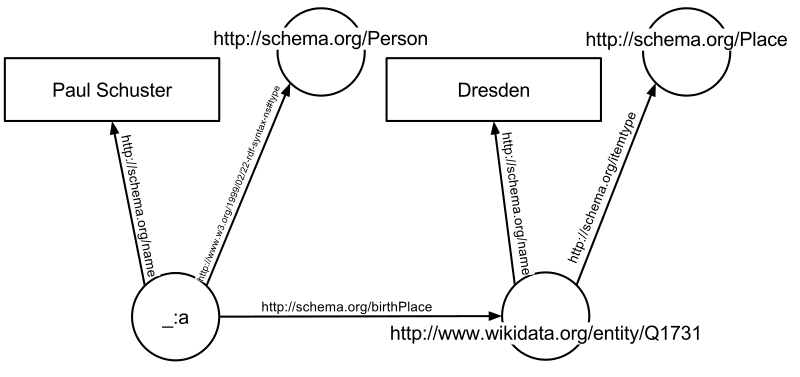
\includegraphics[scale=0.40]{imagens/rdf_example1.png}
	\caption{Exemplo do grafo RDF \citep{RDFWikiImage}}
	\label{fig:rdf_graph}
\end{figure}

\begin{figure}
	\centering
	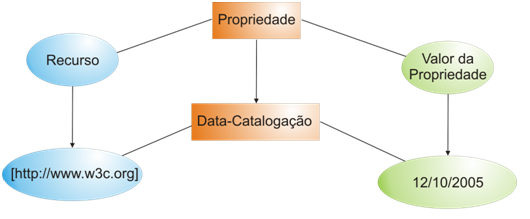
\includegraphics[scale=0.65]{imagens/rdf_example2.png}
	\caption{Exemplo do grafo da tripla sujeito predicado objeto \citep{WebSemanticaDevmedia}}
	\label{fig:rdf_graph2}
\end{figure}

O uso da URI é especialmente notável para a Web, uma vez que não é possível apenas se basear em valores literais, mesmo para representar um atributo de algo, já que é desejado ter a definição e estrutura podendo considerar um domínio em específico. Como exemplo, com uma URI é possível identificar de forma única o predicado “título” que se refere ao título da função em uma empresa, e não um título de filme. Então, a tripla forma um grupo de três entidades que expressam uma declaração sobre o dado semântico, na forma de “sujeito, predicado, objeto”. Com essa estrutura de links é formado um grafo direcionado, com \textit{labels}, aonde suas arestas representam o link nomeado entre dois recursos representados pelos seus nós \citep{W3CRDF}.

\subsection{SPARQL}

O SPARQL é uma linguagem de consulta para o grafo do RDF \citep{SparqlW3C}. Dessa forma, pode-se criar \textit{queries} através de diversos conjuntos de dados de triplas, podendo ser aplicado uma série de filtros para limitar e ordenar os resultados retornados. Diferentemente das linguagens de consulta de banco de dados relacionais, o objeto da coluna não é homogêneo, ou seja, o tipo dado da célula da tabela de resultados é implicado ou definido pelo predicado informado através da URI. O sujeito do RDF pode ser classificado com um análogo a uma entidade nos bancos de \ac{SQL}, diferindo onde os campos (ou atributos) são representados como predicados e/ou objetos separados.

O exemplo do Código Fonte \ref{cod:sparql-example} demonstra a consulta de dados de uma ontologia \textit{foaf}\footnote{http://xmlns.com/foaf/spec/}, conhecida como "friend of a friend".

\begin{lstlisting}[caption=Exemplo de consulta na linguagem SPARQL, language=SPARQL, frame=single, label={cod:sparql-example}, float, numbers=left]
PREFIX foaf: <http://xmlns.com/foaf/0.1/>
PREFIX rdf: <http://www.w3.org/1999/02/22-rdf-syntax-ns#>
SELECT ?name 
       ?email
WHERE
  {
    ?person  a          foaf:Person .
    ?person  foaf:name  ?name .
    ?person  foaf:mbox  ?email .
  }
}
\end{lstlisting}

\subsection{OWL}

Ontology Web Language é uma linguagem para definir e instanciar ontologias na Web \citep{OWLW3C}. Um programa que deseja comparar ou combinar informações entre dois bancos de dados com URIs distintas, deve saber se termos podem ser usados para descrever o significado da mesma coisa \citep{bernerslee2001semantic}. O objetivo é que um programa descubra o significado comum seja para o que for encontrado entre os conjuntos de dados. A solução proposta na Web Semântica para esse problema é a utilização de uma coleção de informações denominadas de ontologias. Na filosofia uma ontologia tem por objeto o estudo das propriedades do ser, tratando da natureza da existência. Entretanto, no campo da inteligência artificial e na Web, é definido como os termos básicos e relações que compreendem um vocabulário de um domínio, bem como regras para combiná-los junto com relações para definir extensões desse vocabulário \citep{Patil:1992:DKS:3087223.3087302}.

Em essência a ontologia é um documento que define formalmente as relações entre termos. As ontologias podem ser vistas de forma semelhante à hierarquia de classes na programação orientada a objetos. Tipicamente uma ontologia para a Web possui uma taxonomia e um conjunto de regras de inferência. A taxonomia define classes (ou conceitos) de objetos e suas relações, sendo assim, um endereço pode ser definido como um tipo de localidade e o código de uma cidade pode ser definido para ser aplicado apenas a localizações, entre outros exemplos.

A linguagem OWL provê três sublinguagens, OWL Lite, OWL DL, OWL Full como apresentado pela \cite{OWLW3C}.

\begin{itemize}
	\item{\textbf{OWL Lite}: Para a criação hierárquica e simples de limitações de \textit{features}. Como exemplo, é possível oferecer suporte a limitações de cardinalidade que só permitam valores de 0 ou 1. É mais simples de prover suporte.} 

	\item{\textbf{OWL DL (descrição lógica)}: Oferece suporte a uma expressividade máxima sem perder a completude computacional (todas as implicações são garantidas para serem computadas), decidibilidade (todos os cálculos finalizaram em um tempo finito). Inclui todas as construções com restrições e separação de tipos (uma classe também não pode ser indivíduo ou propriedade, uma propriedade também não pode ser um indivíduo ou uma classe).}

	\item{\textbf{OWL Full}: Oferece o máximo de expressividade e é sintaticamente livre do RDF sem garantias computacionais. Nessa linguagem uma classe pode ser tratada simultaneamente como uma coleção de indivíduos ou indivíduo como todo. Então, a OWL Full permite uma ontologia ter seu significado ampliado ao pré-definido (RDF ou OWL) vocabulário.}
\end{itemize}

Todas as sub-linguagens são extensões de sua predecessora, sendo assim cada ontologia válida em OWL Lite é uma ontologia válida em OWL DL que por sua vez é uma ontologia válida em OWL Full \citep{OWLW3C}. É notável destacar que o inverso das relações não é verdadeiro. Completando, todo documento OWL é um documento em XML construído com o RDF.

\subsubsection{Estrutura de um documento:}

Com a OWL é possível descrever de forma natural classes e relacionamentos entre documentos e aplicações na Web \citep{OWLReport:2005}. Os termos descritos devem estar dispostos de tal maneira que não cause ambiguidade, assim é necessário que seja informado quais vocabulários serão empregados. Para o uso de vocabulários a \cite{OWLW3C} informa que deve-se definir no topo do documento os \textit{xml namespaces} \footnote{No XML, os namespaces são nomes únicos para elementos e atributos no documento. Para resolver as ambiguidades e facilitar as referências antes dos nomes são utilizados prefixos}, conforme mostrado no código fonte \ref{cod:owl-prefixes}.

\begin{lstlisting}[caption=Exemplo do topo de um documento OWL, language=XML, frame=single, label={cod:owl-prefixes}, float, numbers=left]
<rdf:RDF 
    xmlns     ="http://www.w3.org/TR/2004/REC-owl-guide-20040210/wine#" 
    xmlns:vin ="http://www.w3.org/TR/2004/REC-owl-guide-20040210/wine#"       
    xml:base  ="http://www.w3.org/TR/2004/REC-owl-guide-20040210/wine#"       
    xmlns:food="http://www.w3.org/TR/2004/REC-owl-guide-20040210/food#"    
    xmlns:owl ="http://www.w3.org/2002/07/owl#"
    xmlns:rdf ="http://www.w3.org/1999/02/22-rdf-syntax-ns#"
    xmlns:rdfs="http://www.w3.org/2000/01/rdf-schema#"
    xmlns:xsd ="http://www.w3.org/2001/XMLSchema#">
\end{lstlisting}

Acrescentando, a \ac{W3C} recomenda incluir no documento um cabeçalho XML que preceda as definições das ontologias como apresentado no código fonte \ref{cod:owl-head}

\begin{lstlisting}[caption=Exemplo do cabeçalho XML de um documento OWL, language=XML, frame=single, label={cod:owl-head}, float, numbers=left]
<!DOCTYPE rdf:RDF [
    <!ENTITY vin  "http://www.w3.org/TR/2004/REC-owl-guide-20040210/wine#" >
    <!ENTITY food "http://www.w3.org/TR/2004/REC-owl-guide-20040210/food#" > ]>
\end{lstlisting}

\begin{lstlisting}[caption=Exemplo de propriedades transitivas no OWL, language=XML, frame=single, label={cod:owl-props}, float, numbers=left]
<owl:ObjectProperty rdf:ID="subordinate">
    <rdf:type rdf:resource="&owl;TransitiveProperty"/>
    <rdfs:domain rdf:resource="#Agent"/>
    <rdfs:range rdf:resource="#Agent"/>
</owl:ObjectProperty>

<Agent rdf:ID="Joao">
    <subordinate rdf:resource="#Pedro"/>
</Agent>

<Agent rdf:ID="Pedro">
    <subordinate rdf:resource="#Maria"/>
</Agent>
\end{lstlisting}

\begin{lstlisting}[caption=Exemplo do cabeçalho de uma ontologia, language=XML, frame=single, label={cod:owl-ontology-head}, float, numbers=left]
<owl:Ontology rdf:about=""> 
  <rdfs:comment>An example OWL ontology</rdfs:comment>
  <owl:priorVersion rdf:resource="http://www.w3.org/TR/2003/PR-owl-guide-20031215/wine"/> 
  <owl:imports rdf:resource="http://www.w3.org/TR/2004/REC-owl-guide-20040210/food"/> 
  <rdfs:label>Wine Ontology</rdfs:label>
  ...
\end{lstlisting}

Por último será informado o cabeçalho da ontologia junto a suas propriedades. Nesse cabeçalho é importante fornecer informações sobre ela própria. Para descrevê-las utiliza-se as propriedades do OWL, uma vez que a ontologia é um recurso, assim demonstrado no código fonte \ref{cod:owl-ontology-head}

Dentro da definição da ontologia poderão ser informados as classes e indivíduos relacionados como as propriedades e suas relações. As propriedades podem ser descritas como transitivas, simétricas, funcionais ou inversamente funcional. Como exemplo, numa propriedade transitiva de subordinado, se é dito que João é subordinado de Pedro e Pedro é subordinado de Maria, portanto João é subordinado de Maria. No código fonte \ref{cod:owl-props} é demonstrado a declaração desse tipo de propriedade.

\subsection{Estrutura na rede semântica}

\begin{figure}
	\centering
	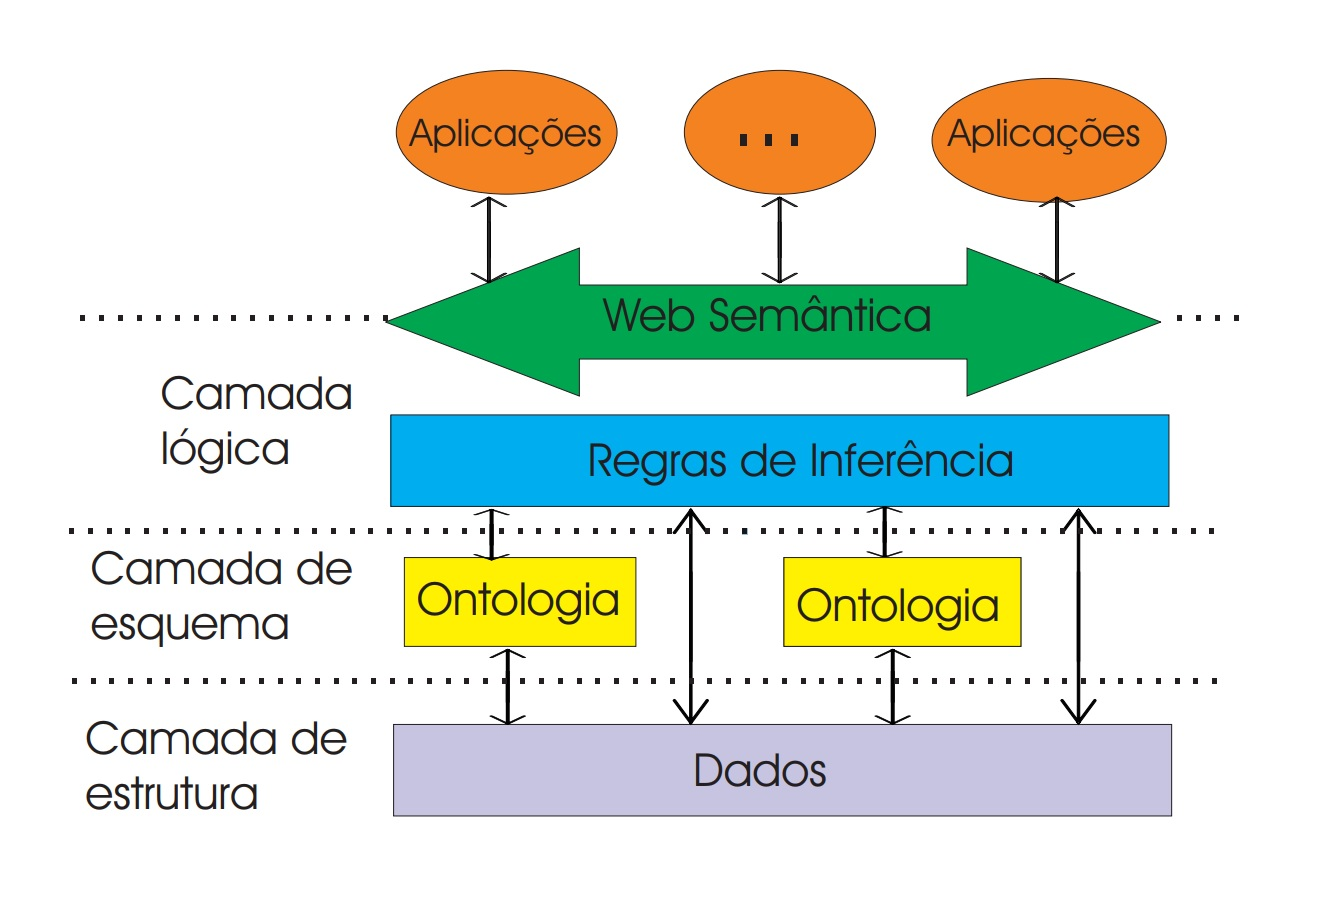
\includegraphics[scale=0.35]{imagens/sw_layers.jpg}
	\caption{Camadas na rede semântica. \citep{OWLReport:2005}}
	\label{fig:sw-layers}
\end{figure}

\begin{figure}
	\centering
	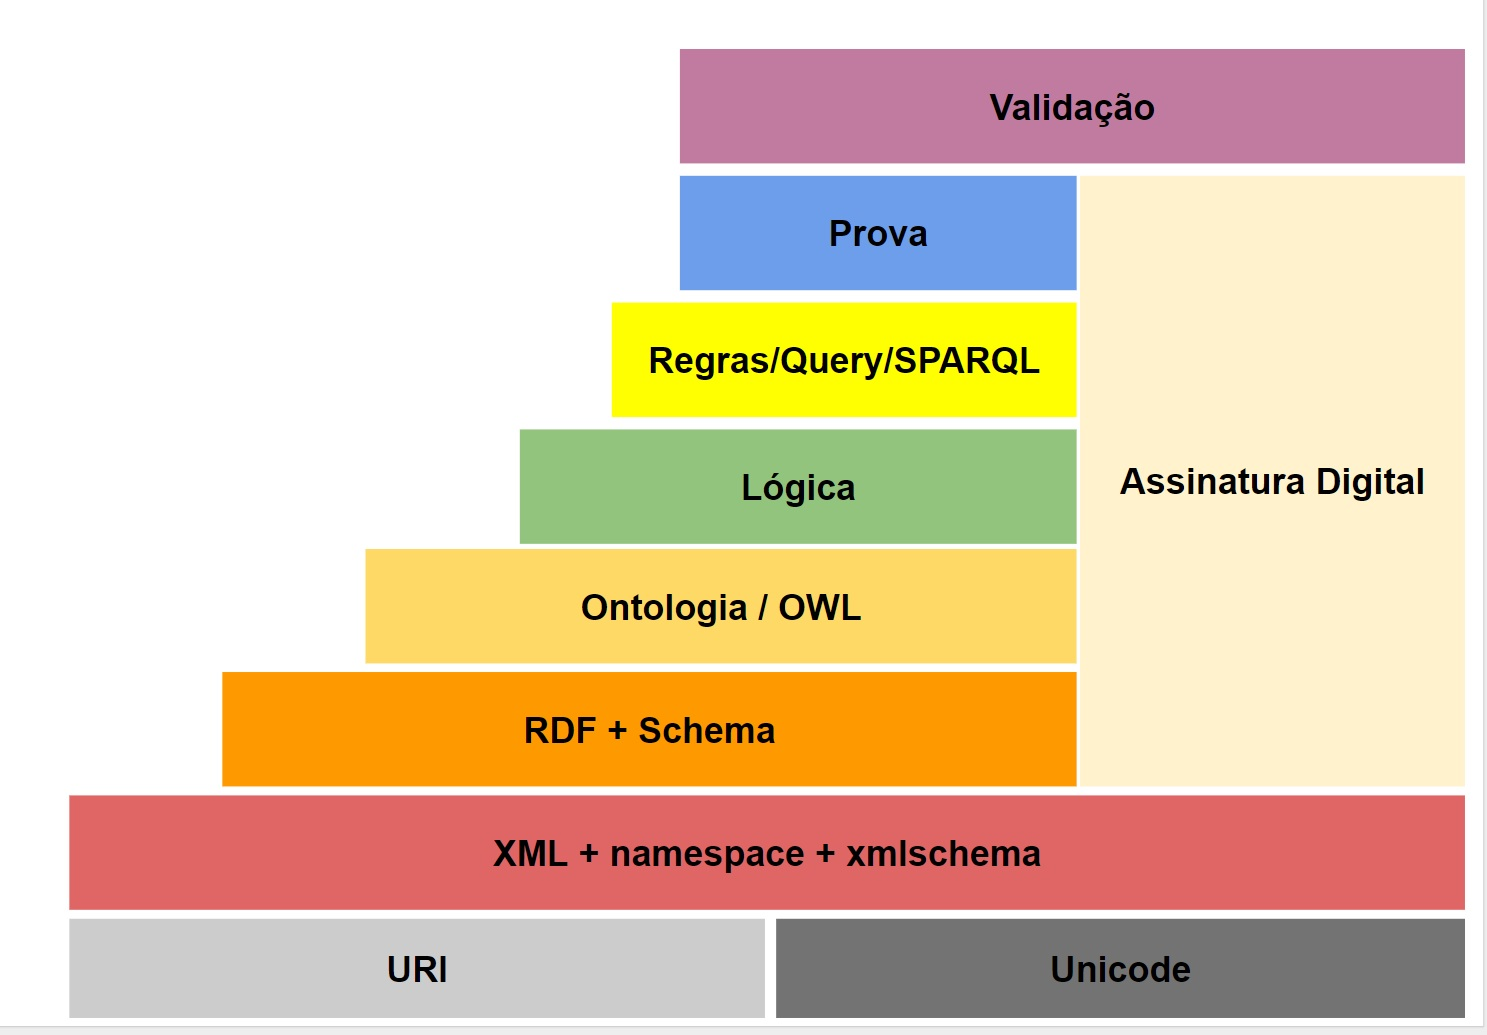
\includegraphics[scale=0.30]{imagens/sw_w3c_stack.jpg}
	\caption{Camadas na rede semântica. Figura elaborado pelo autor de acordo com a publicação de \cite{SemanticWebStack}}
	\label{fig:sw-w3c-stack}
\end{figure}

A introdução das tecnologias para alcançar os princípios idealizados na Web Semântica são implantados em camadas. De acordo com \cite{bernerslee2001semantic} é possível dividir esses serviços em três grandes camadas, como demonstrado na figura \ref{fig:sw-layers}. Na camada de estrutura os dados são organizados e definidos seus significados, na qual utiliza-se as triplas do RDF. A camada com os esquemas estão as ontologias, utilizando-se o OWL para a representação de conceitos, inferências através das taxonomias e conjunto de regras. Por último na camada lógica é definida para fazer inferência sobre os dados. Dessa forma, o desenvolvimento dessas tecnologias (ainda em andamento) e padronização dos formatos foi formulado pela W3C como uma pilha das camadas \citep{SemanticWebStack} da Web Semântica confiável, conforme mostrado na figura \ref{fig:sw-w3c-stack}.

\section{Dados ligados}

A evolução da WWW tornou cada vez mais acessível a publicação e acesso a documentos pela navegação no espaço global, através links dos hipertextos \citep{Bizer2009}. Com os navegadores da Web pode-se passear pelos links nesse espaço e em especial com o uso dos buscadores, que indexam páginas para facilitar a recuperação. Tais mecanismos já estão amplamente difundidos na publicação de documentos, mas quando comparados aos dados\footnote{Note que embora os termos "dados" e "documentos" possam ser análogos, no contexto da Web, documentos tratam-se das páginas dos sites e dados, de fato a informação em si. Assim, na Web os documentos apenas objetivam o aspecto da apresentação não contento a semântica dos dados presentes.} em si, esses princípios ainda foram timidamente aplicados. Assim, com o crescimento da Web Semântica trouxe-se a ênfase em criar uma Web para os dados, capaz descrever entidades individuais presentes nos documentos, conectando-se por links categorizados para relacionar tais entidades. O objetivo não é somente colocar dados na Web, mas utilizar links que ambas máquinas (principalmente) e humanos possam navegar.

Suportando essa evolução da Web \citep{LinkedData:2006} introduziu um conjunto de melhores práticas para a publicação e conexão de dados estruturados na Web, denominado de \textit{Linked Data} (dados ligados). A adoção dessas práticas permite a extensão da Web como um espaço de dados global conectado de diversos domínios, desde pessoas, livros, publicações até dados governamentais dos mais variados assuntos. Com essa Web de dados surge a oportunidade para novos tipos de aplicações \citep{Bizer2009}, como navegadores customizados para um determinado domínio podendo saltar entre diferentes fontes de dados.

Resumidamente, a \cite{LinkedDataW3C} define que para a Web dados ser uma realidade é necessário que os dados estejam disponíveis em padrões de formatos que sejam buscáveis e manipuláveis pelas ferramentas e tecnologias da Web Semântica. Complementando, é preciso também ter acesso ao relacionamento de dados. O conjunto de \textit{datasets} inter-relacionados na Web, para criar links tipificados entre dados de diferentes fontes é o que se denomina de dados ligados.

Ao contrário dos documentos \ac{HTML} na Web dos hipertextos, os dados ligados se baseiam-se nos documentos contendo dados em RDF. Assim são construídos links que são tipificados para realizar declarações sobre coisas arbitrárias no mundo. \cite{LinkedData:2006} enumerou um conjunto das regras para a publicação e conexão dos dados, conhecidos como os princípios dos dados ligados:

\begin{enumerate}
	\item{Usar URIs para nomear coisas}
	\item{Usar \ac{HTTP} URIs para que pessoas possam procurar seus nomes.}
	\item{Quando alguém procura uma URI, forneça informação útil, utilizando os padrões como RDF e SPARQL.}
	\item{Inclua links para outras URIs, para que assim eles possam descobrir mais coisas.}	
\end{enumerate}

Um exemplo notável do uso das dados ligados, é o projeto da DBPedia\footnote{ http://wiki.dbpedia.org} que essencialmente torna o conteúdo da Wikipedia\footnote{https://www.wikipedia.org} disponível em RDF.

\subsection{Linked Open Data}

Posteriormente em 2010, para incentivar o uso dados ligados no meio governamental, \cite{LinkedData:2006} desenvolveu um "sistema de avaliação" dos dados ligados. O objetivo era expandir o termo introduzindo os dados abertos, onde fossem publicados sob uma licença que não impede o livre reuso. No sistema de avaliação consta um esquema de pontuação em estrelas de 1 a 5, onde cada estrela a mais também acumula as definições das estrelas anteriores, conforme consta na figura \ref{fig:lod-rating}.

O \ac{LOD} tornou-se o projeto de maior adoção dos princípios dos dados ligados \citep{Bizer2009}, sendo um esforço colaborativo iniciado em 2007 para suportar as definições e tecnologias da Web Semântica introduzidas pela W3C. O motim para o início da colaboração era de mapear os dados da Web identificando os conjuntos que já estavam disponíveis sob licença aberta. O projeto inclui dados de várias fontes, como a Wikipedia\footnote{https://www.wikipedia.org}, Geonames\footnote{http://www.geonames.org}, Wordnet\footnote{https://wordnet.princeton.edu} entre diversos outros de múltiplos domínios, alcançando um impressionante diagrama como mostrado na figura \ref{fig:lod-graph}.

\begin{figure}
	\centering
	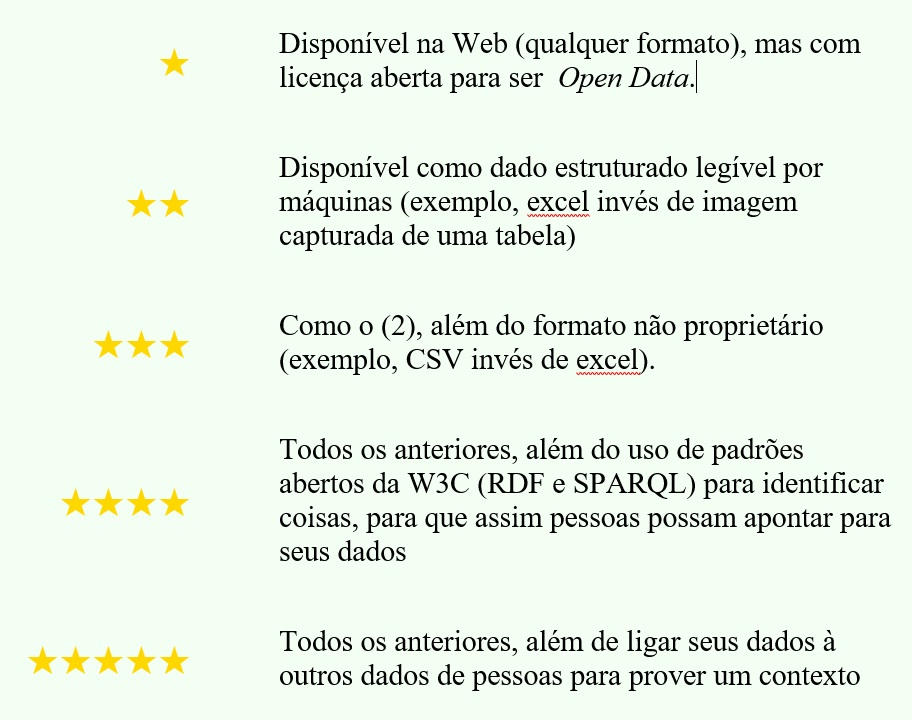
\includegraphics[scale=0.50]{imagens/lod_rating.jpg}
	\caption{Sistema de avaliação do LOD \citep{SemanticWebStack}}
	\label{fig:lod-rating}
\end{figure}

\begin{figure}
	\centering
	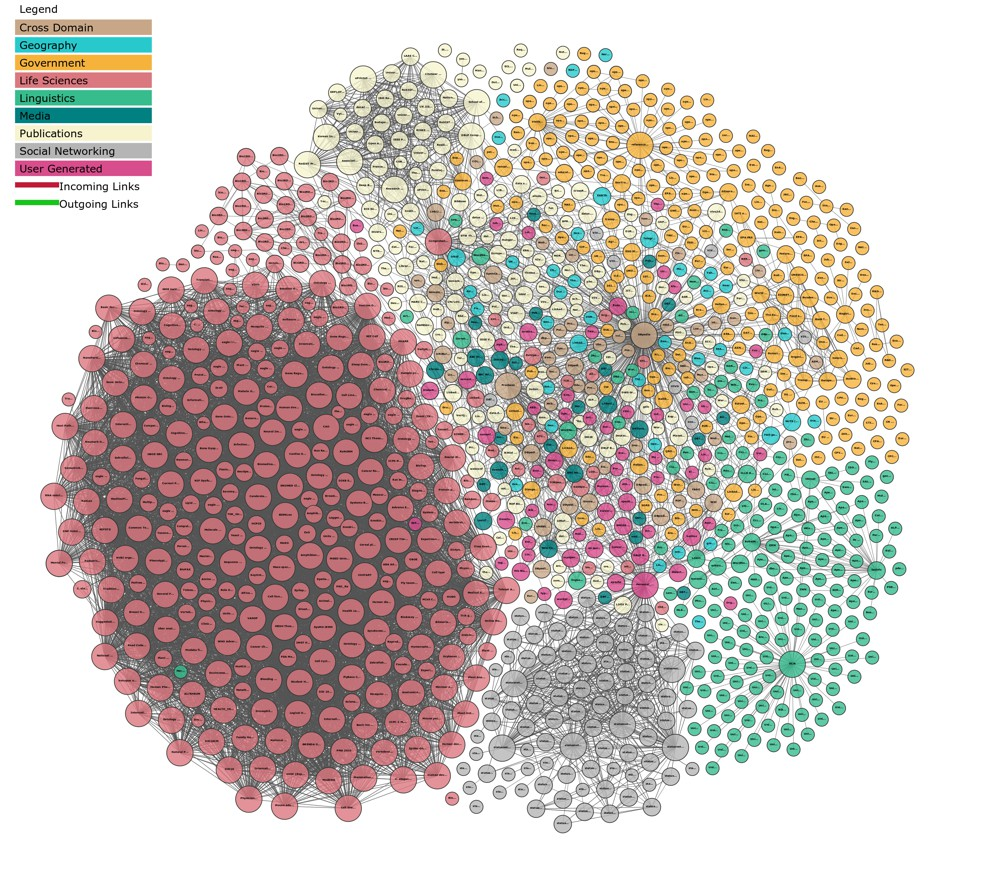
\includegraphics[scale=0.47]{imagens/lod_graph.jpg}
	\caption{Diagrama da nuvem dos dados ligados \citep{LODGraph}}
	\label{fig:lod-graph}
\end{figure}

\section{Similaridade Semântica}

A similaridade semântica entre dois termos, recursos, itens ou documentos é uma métrica para medir a distância de seus significados ou semântica, dado suas ontologias \citep{Slimani2013}. O objetivo é estabelecer características em comum entre dois conceitos. A distância entre dois conceitos para humanos pode não ter uma definição formal, já que se pode criar um juízo de valor diferente no relacionamento entre eles. Como exemplo, para uma pessoa a maçã e a banana podem estar mais relacionadas do que a maçã e a pera para outra. A similaridade e relação semântica podem por vezes serem determinadas como a mesma coisa, ambas como métricas de distâncias entre termos, contudo a similaridade semântica é mais específica \citep{Slimani2013}. A relação semântica é calculada usando um modelo de espaço vetorial e uma métrica de similaridade, como a similaridade do cosseno \ref{eq:cosine_sim} que dado dois vetores $A$ e $B$ como uma representação de dois documentos e $A_i$ e $B_i$ seus componentes, seja calculado o produto vetorial euclidiano. \citep{Singhal2001}.

\begin{equation}
	A \cdot B = \norm{A}_2 \norm{B}_2 \cos(\theta)
\label{eq:cosine_sim_eu}
\end{equation}

\begin{equation}
	similaridade = \cos(\theta) = \frac{ A \cdot B }{ \norm{A}_2 \cdot \norm{B}_2 }
	= \frac{ \sum_{i=1}^{n} A_i B_i }{ \sqrt{ \sum_{i=1}^{n} A_i^{2} } \sqrt{ \sum_{i=1}^{n} B_i^{2} } }
\label{eq:cosine_sim}
\end{equation}

Entretanto, para a similaridade semântica é levado em consideração relações léxicas de sinonímia e hiperonímia onde o significado é abrangido pelo outro termo mais geral (como carro e veículo) \citep{Gracia2008}. Na prática, a similaridade semântica pode ser medida pelo menor caminho entre dois termos utilizando suas ontologias associadas. Para calcular a similaridade podem ser usadas diversos tipos de ontologias. \cite{Slimani2013} descreve dois principais tipos de ontologias usadas para medir similaridade.

\begin{itemize}
	\item{\textbf{Propósito genérico}: \textit{Wordnet}\footnote{https://wordnet.princeton.edu} é um banco de dados que modela o conhecimento léxico da língua inglesa. Nomes, verbos, adjetivos e advérbios são agrupados em conjuntos sinônimos, onde cada um expressa um conceito distinto. Essa ontologia pode ser utilizada para criar um \textit{score} de similaridade. Pode ser considerada um ontologia para termos de linguagem natural.}
	
	\item{\textbf{De domínio específico}: \textit{ULMS}\footnote{https://www.nlm.nih.gov/research/umls} é um sistema de linguagem médica com uma rede semântica de ontologias de multiuso, multilíngue para biomedicina, conceitos e assuntos relacionados à saúde. O banco de dados do sistema possui uma coleção de vocabulários de conceitos e termos e seus relacionamentos que são denominados de \textit{Metathesaurus}. Cada Metathesaurus é classificado como pelo menos uma categoria semântica.}	
\end{itemize}

\subsection{Medidas de Similaridade Semântica}

Na literatura já foram apresentadas algumas medidas de similaridade semântica, mas comumente existem três fatores principais \citep{Slimani2013} que podem ser associados na topologia (i.e. nós do grafo direcionado) das ontologias: \textit{path length}, \textit{depth}, \textit{density}. Todos esses fatores afetam a medida da distância semântica, assim como as características entre dois termos, que podem aumentar ou diminuir as medidas de acordo com suas semelhanças. Quanto a densidade entre dois termos trata-se do número de filhos dos quais pertencem ao menor caminho (\textit{path}) da raiz ao mais específico conceito entre esses termos. Os fatores que influenciam nas medidas levam a definição de uma classificação que podem ser divididas em quatro principais \citep{Slimani2013}: baseadas em estrutura, conteúdo, recursos ou características e as híbridas que combinam as características estruturais (\textit{path length}, \textit{depth}, \textit{density}) e alguma outra abordagem.

\subsubsection{Baseadas em estrutura:}

As medidas baseadas em estrutura (\textit{Structured-based ou Path-based}, utilizam funções que computam a similaridade baseada na hierarquia e estrutura da ontologia, ou seja, onde um conceito é definido como “é parte de”, “é um” etc. A função calcula o tamanho do caminho que liga os termos e seus posicionamentos no grafo direcionado da ontologia. Quanto mais dois conceitos são similares, mais \textit{links} existem entre eles. Dentre as medidas baseadas em estrutura se destacam:

\begin{itemize}
	\item{\textbf{\textit{Shortest Path} \citep{Rada:1989}}: A medida do menor caminho é um tipo de medida de distância que é primariamente voltada para lidar com hierarquias em redes semânticas. A função da similaridade entre conceitos $C_1$ e $C_2$ é definida como:

	\begin{equation}
		Sim(C_1, C_2) = 2 * Max(C_1, C_2) - SP	
	\label{eq:shortest_path}
	\end{equation}
	
	A função $Max$ é o maior tamanho do caminho entre $C_1$ e $C_2$, quanto a $SP$ é menor caminho relacionando os dois conceitos.}
	
	\item{\textbf{\textit{Weighted Links}}: Similar a medida do menor caminho, contudo é introduzido um conceito de pesos para os links entre os conceitos a serem comparados.}
	
	\item{\textbf{\cite{Wu:1994}}: Para essa medida sejam dois conceitos $C_1$ e $C_2$, é levado em consideração a noção intuitiva de que quanto maior a profundidade, mais similares os conceitos são. Na função tem-se que $N_1$ e $N_2$ são a quantidade de links da forma "é um" de $C_1$ e $C_2$, onde o conceito mais específico é o mais próximo ancestral  $C$ entre eles. 

	\begin{equation}
		Sim_{W \& P}(C_1, C_2) = \frac{2H}{N_1 + N_2 + 2H}	
	\label{eq:wu_palmer}
	\end{equation}	}	
\end{itemize}

\subsubsection{Baseadas em conteúdo:}

As medidas baseadas no conteúdo, são aquelas que utilizam a informação do conteúdo para medir similaridade. O conteúdo de um conceito é definido pela frequência de termos dado uma coleção de documentos. Grande parte das medidas deste tipo utilizam a informação compartilhada de dois conceitos pais $C_1$ e $C_2$, dos qual $S(C_1; C_2)$ é o conjunto de conceitos que os engloba, conforme a equação \ref{eq:mis}.  O menor $p(C)$ é utilizado quando há mais de um pai em comum que $C$ é o \ac{MIS}, ou seja, o conceito mais informacional que os engloba.

	\begin{equation}
		P_{mis}(C_1, C_2) = min_{C \in S(C_1;C_2)} \{p(C)\}
	\label{eq:mis}
	\end{equation}

Algumas das medidas deste tipo são:

\begin{itemize}

	\item{\textbf{\cite{Resnik:1999}}: O principio desta medida define que dois conceitos são mais similares se eles possuem mais informações compartilhadas. A informação compartilhada entre $C_1$ e $C_2$ é o conteúdo de conceitos que os engloba no grafo. A definição de \textit{Resnik} define a medida como a seguinte equação:
	
	\begin{equation}
		Sim_{Resnik}(C_1, C_2) = - \ln (p_{mis}(C_1, C_2))
	\label{eq:resnik}
	\end{equation}}
	
	\item{\textbf{\cite{Lin1993PrincipleBasedPW}}: A proposta é incorporar o vetor semântico e a ordem das palavras para calcular a similaridade. A medida combina o menor caminho $SP$ entre dois conceitos e a profundidade $N$ da taxonomia em relação ao conceito $C$ mais em comum. A definição da equação segue conforme abaixo:

	\begin{equation}
		Sim_{Li}(C_1, C_2) = \mathrm{e}^{-\alpha * SP} * \frac{ \mathrm{e}^{\beta * N} - \mathrm{e}^{- \beta * N} }{ \mathrm{e}^{\beta * N} + \mathrm{e}^{- \beta * N} }
	\label{eq:li}
	\end{equation}}
	
\end{itemize}

\subsubsection{Baseadas em características ou recursos:}

Baseia-se em características ou recursos (\textit{Featured-based}), que partem do princípio de valorizar informações importantes em relação ao conhecimento sobre um termo. A medida assume que os conceitos são descritos por termos indicando suas propriedades ou \textit{features}. A similaridade entre dois conceitos é definida por uma função (\ref{eq:tversky}) que relaciona suas propriedades ou relacionamentos a outros termos similares na hierarquia da ontologia. \cite{Tversky:1977} apresenta uma medida \textit{Feature-based} de termos para calcular a similaridade entre diferentes conceitos, contudo o posicionamento desses termos na taxonomia e a informação do conteúdo não são levadas em consideração. A proposta é de que com termos descritos por um conjunto de palavras como propriedades do conceito, então as que são em comum tendem a aumentar a similaridade, enquanto as que não são em tendem a diminuí-la. Dessa forma, é definida uma equação onde $C_1$ e $C_2$ representam o conjunto de descrições dos termos e $\alpha \in [0,1]$ é a relação de relevância das características que não são em comum. O valor de $\alpha$ aumenta o quão mais em comum dois conceitos são, e decresce com suas diferenças, e não é necessariamente uma relação de simetria, mas mais baseada na similaridade \citep{Slimani2013}.

\begin{equation}
	Sim_{Tversky}(C_1, C_2) = \frac{ |C_1 \cap C_2| }
	{ |C_1 \cap C_2| + \alpha |C_1 - C_2| + (\alpha - 1)|C_2 - C_1| }
\label{eq:tversky}
\end{equation}

\section{Projetos na Web Semântica}

\subsection{DBPedia}

A DBPedia (DB para \textit{database}) é um esforço colaborativo para a extração de dados do Wikipedia para publicação de dados essencialmente em RDF \citep{Auer:2007:DNW:1785162.1785216}. Um dos objetivos é possibilitar que outros explorem a criar uma experiência da enciclopédia mais abrangente, utilizando serviços e aplicações na Web Semântica. O projeto é um dos mais famosos que aplica os conceitos de dados ligados, onde sua importância não somente é dada pela publicação dos dados da Wikipedia, mas também da incorporação de links de outros \textit{datasets}. De fato, o DBpedia, por muitas vezes é considerado um núcleo dentro da iniciativa do LOD.

O projeto tem o foco em converter o conteúdo presente do Wikipedia em conhecimento estruturado utilizando as tecnologias da Web Semântica, para que outros agentes possam explorar realizando consultas e ligando a outros conjuntos de dados \citep{Auer:2007:DNW:1785162.1785216}. Assim, o projeto cobre uma das limitações da Wikipedia que é a dependência de apenas ter a busca em texto livre para encontrar informação. Desse papel, o projeto promove três importantes contribuições:

\begin{itemize}
	\item{Desenvolvimento de um \textit{framework} para extração de informação, o qual converte o conteúdo da Wikipedia em RDF.} 

	\item{Prover o conteúdo da Wikipedia como um largo, multi-domínio \textit{dataset} de RDF. São mais de 100 milhões de triplas já mapeadas. A figura \ref{fig:dbpedia-triples} mostra um recorte das entidades mapeadas do DBPedia.}
	
	\item{Interligar o DBpedia com outros conjuntos de dados abertos, o que expande a contagem das triplas RDF para mais de bilhão.}
	
	\item{Desenvolvimento de uma série de interfaces e módulos de acesso para que tal \textit{dataset} possa ser acessado por serviços da Web ligado a outros sites.}	
\end{itemize}

\begin{figure}
	\centering
	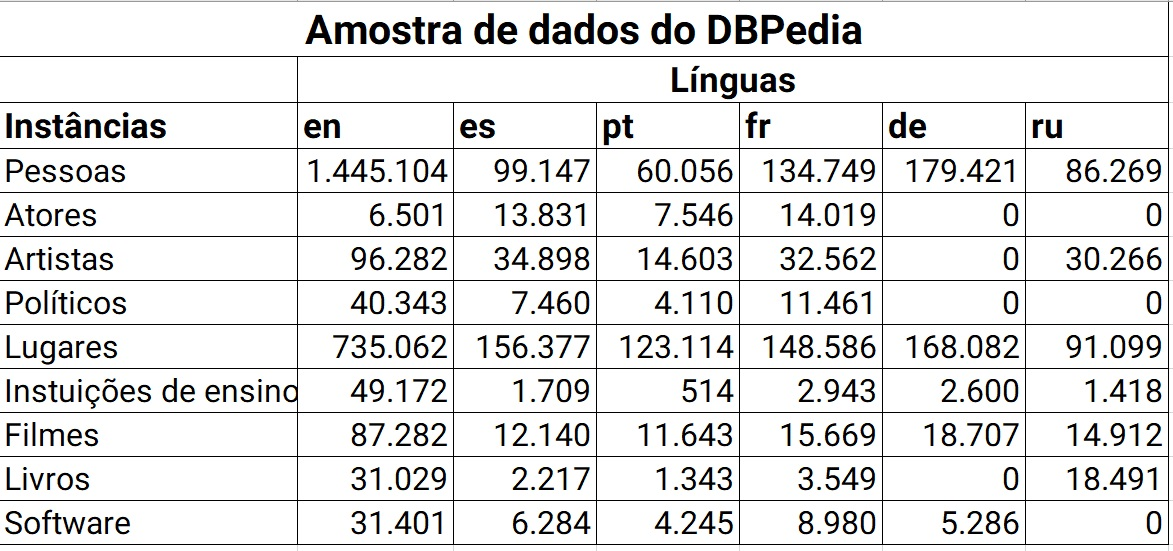
\includegraphics[scale=0.60]{imagens/dbpedia_triples.jpg}
	\caption{Recorte da tabela de dados de triplas de entidades mapeadas no DBPedia. \citep{DBPedia:2014}}
	\label{fig:dbpedia-triples}
\end{figure}

\begin{figure}
	\centering
	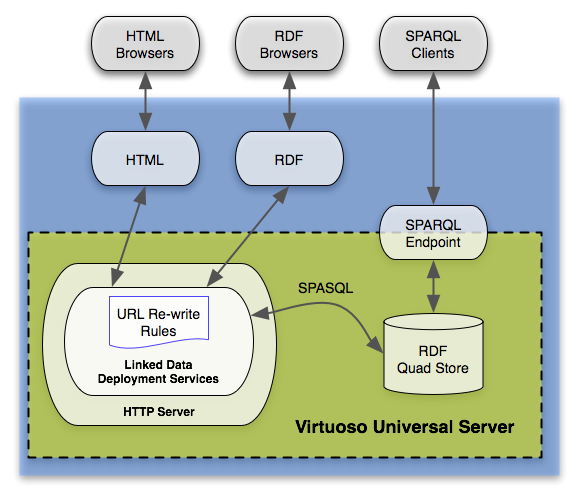
\includegraphics[scale=0.55]{imagens/dbpedia_virtuoso.png}
	\caption{Ilustração da arquitetura do DBPèdia \citep{DBPediaVirtuoso}}
	\label{fig:dbpedia-virtuoso}
\end{figure}

Como a iniciativa compõe o movimento do LOD, os dados do DBpedia podem ser importados por aplicações \textit{third party} utilizando a licença aberta. O projeto faz uso da plataforma do \textit{Virtuoso Universal Server}\footnote{https://virtuoso.openlinksw.com} para prover os dados de RDFs através de uma interface e um \textit{endpoint} em SPARQL. Na figura \ref{fig:dbpedia-virtuoso} é apresentado um panorama da arquitetura do projeto.

\subsection{Google Knowledge Graph}

O \textit{Knowledge Graph} é uma base de conhecimento desenvolvida pelo Google\footnote{https://www.google.com} para melhorar e ampliar seu mecanismo de busca \citep{GoogleKnowledge}. Alinhado aos objetivos da Web Semântica, o projeto pretende expandir o buscador com um grafo de conhecimento, onde foi mapeado entidades de dados legíveis para máquinas com o intuído recuperar a informação semântica nos termos buscados. De forma simples, o intuito é ter a informação de coisas e não de \textit{strings}. Como exemplo, ao ser buscado a palavra "leão", não será apenas retornado uma lista de sites que possuem referências a palavra, mas também prover a semântica e taxonomias envolvidas com a ontologia e relacionados.

\begin{figure}
	\centering
	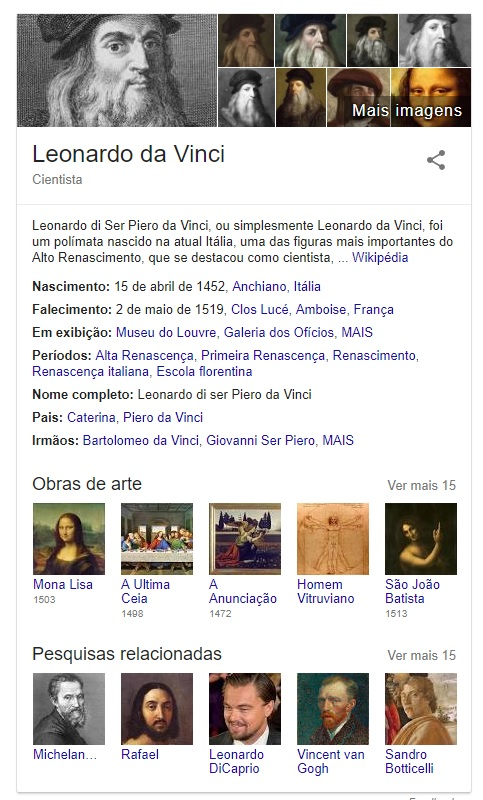
\includegraphics[scale=0.55]{imagens/knowledge_graph.jpg}
	\caption{Ilustração do sumário de dados mapeados no Google Knowledge Graph.}
	\label{fig:knowledge-graph}
\end{figure}

Com \textit{Knowledge Graph} é possível pesquisar por pessoas, lugares, esportes, filmes e diversas informações que o Google mapeou no grafo do conhecimento. O serviço já conta com mais de 500 milhões de objetos e 3.5 bilhões de fatos sobre o relacionamento entre diferentes objetos. O objetivo do Google é ampliar o mecanismo de busca em três sentidos: Possibilitar encontrar o item certo, obter um melhor sumário, ser mais amplo e profundo. Um dos primeiros passos da companhia para atingir os objetivos do projeto é a construção do painel do sumário. Quando pesquisamos por \textit{Leonardo Da Vinci}, procurando seja pelas suas pinturas ou por pintores da renascença, o sistema montará um quadro de dados, conforme a figura \ref{fig:knowledge-graph} com as informações, além trazer itens com relações próximas, como seus quadros e outros artistas relacionados. Com esse tratamento \cite{GoogleKnowledge} alega que será possível melhor compreender o que os usuários buscam, além de dar importantes passos para migrar de um motor informação para um de conhecimento, algo importante para o uso em seus assistentes virtuais.

\section{Sumário}

Neste capítulo, foi apresentado os conceitos que fundamentam o desenvolvimento de sistemas para representação de conhecimentos, assim como a abordagem e objetivos da Web Semântica sobre o tema. Em sequência foram introduzidas as principais tecnologias e princípios que são utilizados e o aprofundamento do significado das ontologias. Também foi abordado um panorama sobre a estrutura das tecnologias utilizadas na Web Semântica. Ainda foi introduzido o princípio e prática dos dados ligados e sua extensão com os dados abertos. Ainda foi exposto um panorama da similaridade semântica e tipos de medidas. Por fim, foram apresentados projetos proeminentes no cenário da Web Semântica. No capítulo \ref{cap:proposal} será discutido os conceitos da proposta do sistema de recomendação implementados neste trabalho.
